\section{Limitations of Perceptrons}

\mode<presentation>{
\begin{frame} 
    \begin{center} \huge
        \secname
    \end{center}
    \begin{center}
    From neurons to neural networks
    \end{center}
\end{frame}
}

\mode<article>{
Connectionist neurons, or perceptrons, are limited in the variety of functions they are able to fit. 
When dealing with classification problems, a perceptron can only find a linear separation between any two classes. Irrespective of the neuron's non-linear activation function, the perceptron is regarded as a \emph{linear classifier}. Whether something falls on one side of the decision boundary or the other, is entirely based on applying a linear filter (i.e. $\vec w^{\top} \vec x$). The non-linearity $f(h)$ merely controls the value range of the neuron's response ($\{0,1\}, (-1,+1)$, \ldots) which helps in interpreting the neuron's response.\\

If observations for two different classes are distributed such that one cannot draw a line to separate them, then the two classes
are not linearly separable. In this case, the perceptron will fail to find a suitable classification boundary between the two classes.
}

\begin{frame}\frametitle{Linear classifiers/linear decision boundaries}

Consider the following binary classification problems with $\vec x \in \R^2$.{}

\question{Can you find a line that separates the two classes for each case?}

\begin{figure}[h]
    \centering
	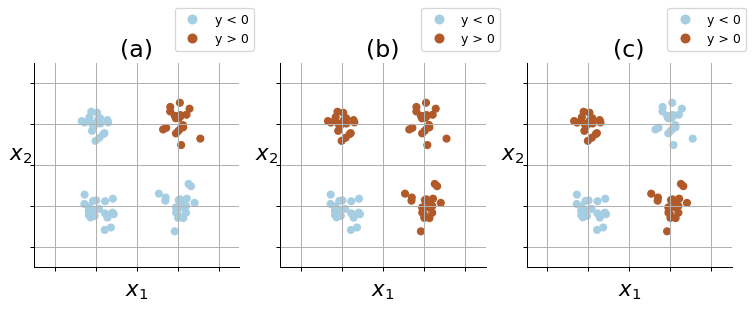
\includegraphics[width=0.8\textwidth]{img/and_or_xor_y}
	\mode<article>{
	\caption{(a) points are classified according to the AND function,
	(b) points are classified according to the OR function,
	(c) points are classified according to the XOR function.
	}
	}
	\label{fig:and_or_xor} 
\end{figure}

\mode<article>{
In \figureref{fig:and_or_xor}, particularly (a) and (b),
it is possible to draw a line that separates the classes. Therefore, the AND and OR functions are linearly separable.
A perceptron is capable of finding such a separating line. However, this does not apply to the third case, for the XOR function.
It is impossible to find a single line that will separate the classes.\\
The XOR function is not linearly separable.
}

\pause 

\question{Can we solve the XOR problem with multiple perceptrons? How?}\\

%\slidesonly{
%\begin{figure}[ht]
     %\centering
	%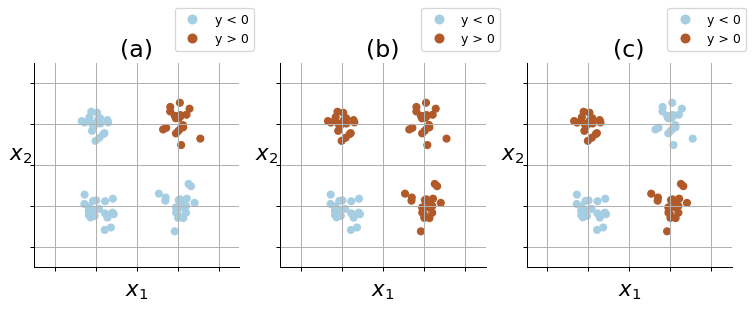
\includegraphics[trim=480 0 0 30, clip, width=0.4\textwidth]{img/and_or_xor_y.png}
	%\caption*{A single perceptron can not solve the XOR problem.}
	%\label{fig:xor} 
%\end{figure}
%}

\pause

\notesonly{
- Yes, think of it as a divide and conquer approach. We split the XOR problem into multiple sub-problems. 
A perceptron is used to solve each sub-problem.

If you're familiar with Boolean algebra, you might recognize the following expression for the XOR function:
}
\mode<presentation>{
\vspace{-10mm}
}

\begin{equation}
\label{eq:xor}
\mathrm{XOR}(x_1, x_2) = 
({\color{magenta}\,{x_1} \; \mathrm{AND} \; \overline{x}_2 \,})
 \;\; \mathrm{OR} \;\; 
({\color{green}\, \overline{x}_1 \; \mathrm{AND} \; x_2 \,})
\end{equation}

\end{frame}

\begin{frame}{Inversion/NOT-Gate}

\begin{center}
\begin{minipage}{0.9\textwidth}

\begin{center}
\begin{minipage}{0.45\textwidth}
	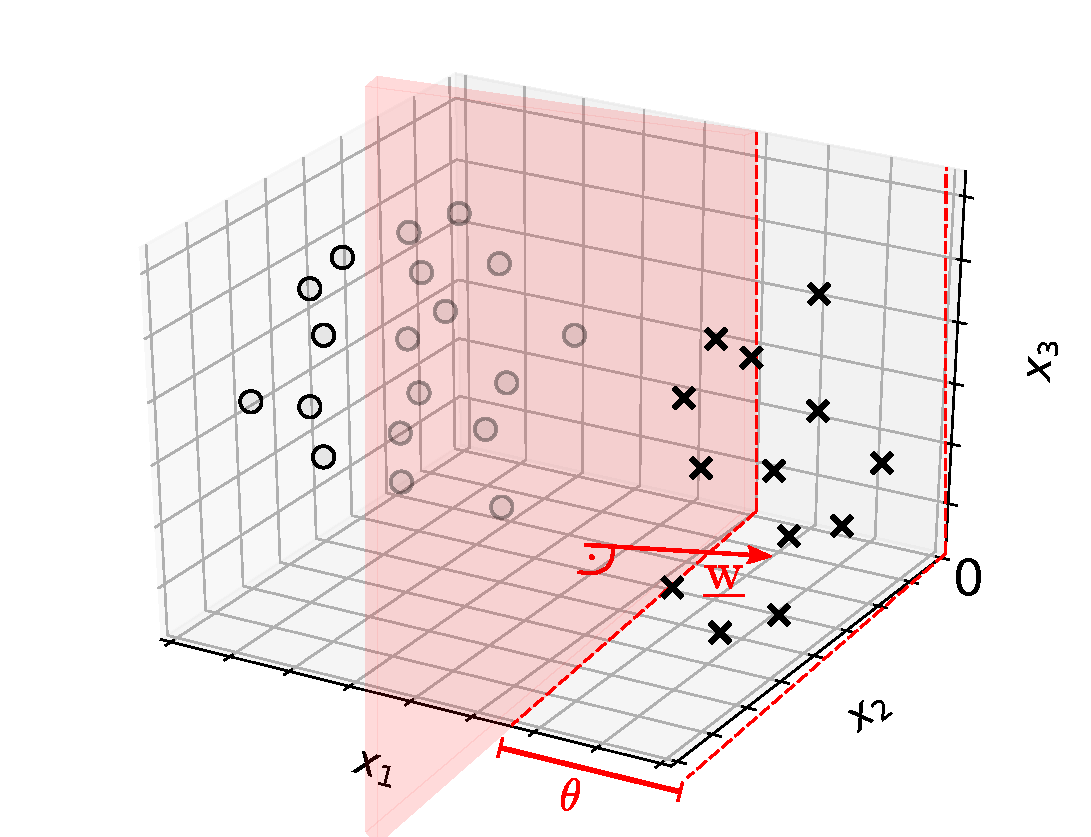
\includegraphics[width=0.9\textwidth]{img/neuron_3d_grid_hyperplane}
\end{minipage}
\begin{minipage}{0.45\textwidth}
	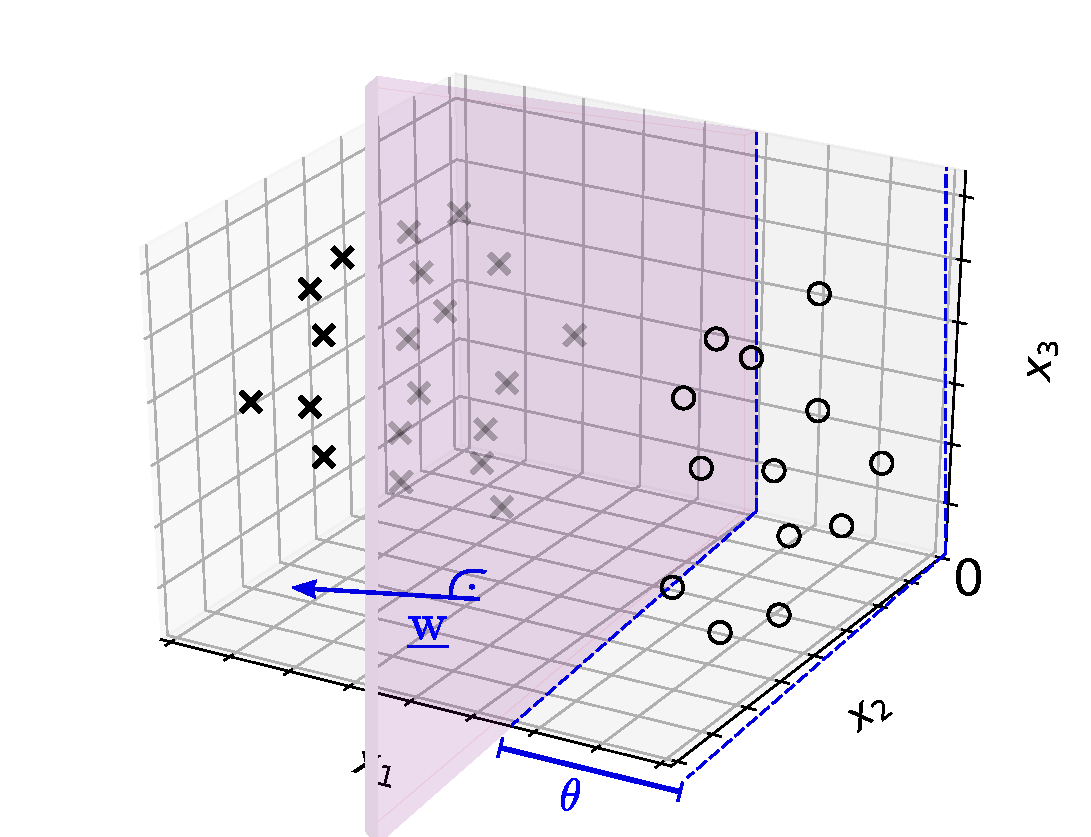
\includegraphics[width=0.9\textwidth]{img/neuron_3d_grid_hyperplane_flip}
\end{minipage}

\end{center}
\end{minipage}
\captionof{figure}{Inverting a neuron's response by flipping the hyperplane}
\end{center}

\end{frame}


\mode<article>{
For instance, the first perceptron ${\color{magenta}s^1_1}$ is tasked to separate the bottom-right cloud of points from the rest. 
A second perceptron ${\color{green}s^1_2}$ is used to separate the top-left cloud from the rest.
A third perceptron ${\color{blue}s^2_1}$ will then use the responses of both and respond to ``is \textbf{only one} of the two perceptrons \textbf{on}?''.

\figref{fig:build_xor} illustrates this approach. One need only recognize that each sub-problem is linearly separable.\\
}

\begin{frame}

\slidesonly{
\begin{equation}
\label{eq:xor}
\mathrm{XOR}(x_1, x_2) = 
({\color{magenta}\,{x_1} \; \mathrm{AND} \; \overline{x}_2 \,})
 \;\; \mathrm{OR} \;\; 
({\color{green}\, \overline{x}_1 \; \mathrm{AND} \; x_2 \,})
\end{equation}
}

\begin{figure}[ht]
    \centering
	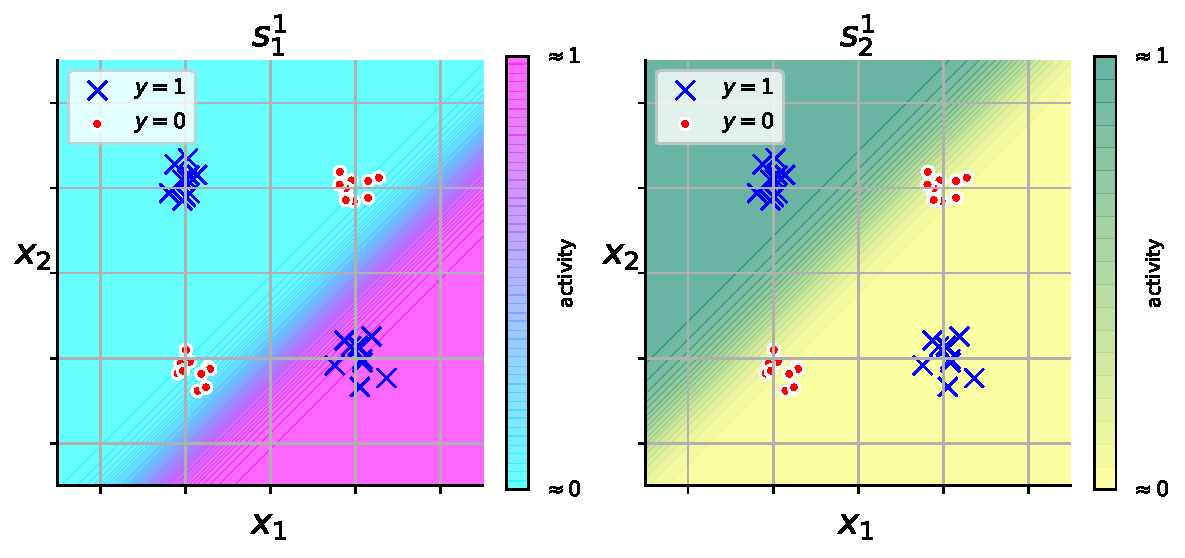
\includegraphics[width=0.75\textwidth]{img/build_xor_crf}
	\caption{Solving sub-problems of the XOR problem.}
	\label{fig:build_xor} 
\end{figure}

\end{frame}

\begin{frame}

\begin{figure}[ht]
    \centering
	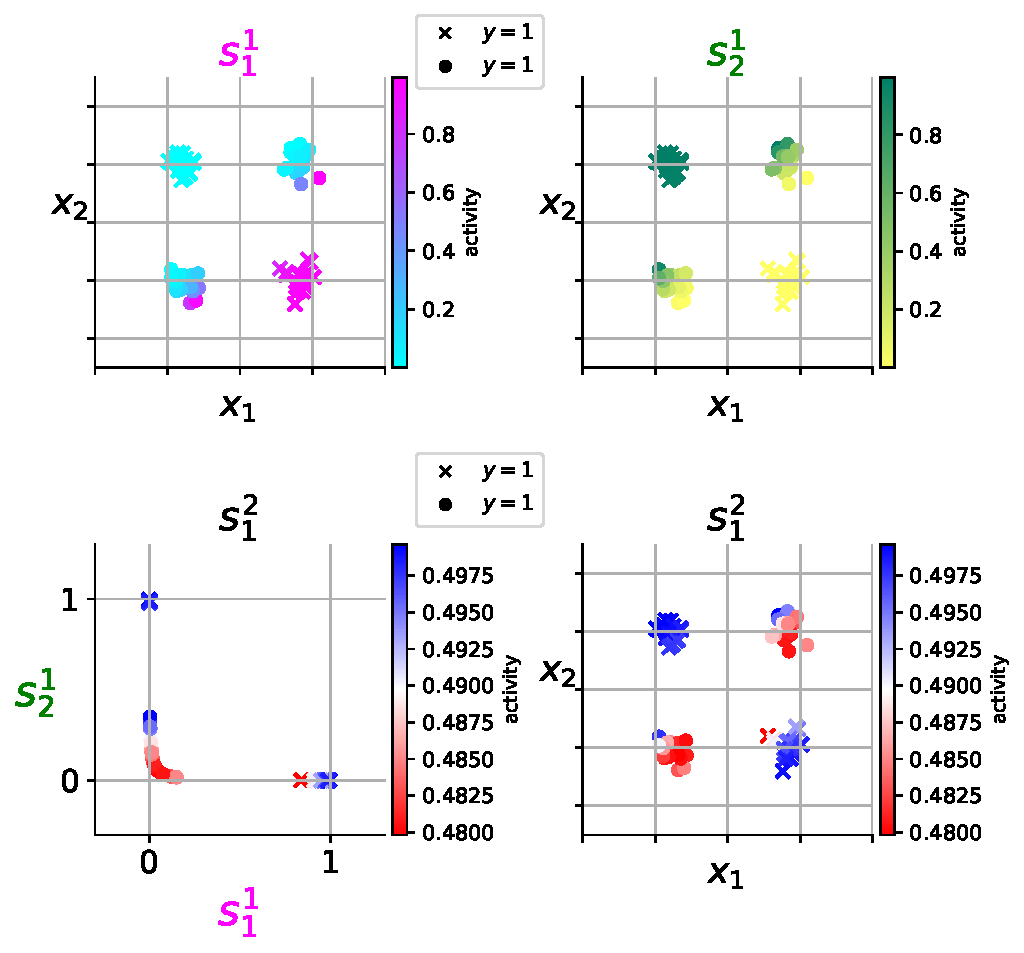
\includegraphics[width=0.75\textwidth]{img/build_xor}
	\caption{Solving sub-problems of the XOR problem.}
	\label{fig:build_xor} 
\end{figure}

\end{frame}


\mode<article>{
\figref{fig:xor_decisions} visualizes the response of the final neuron $s^2_1$ for different values of $x_1$ and $x_2$. The space is partitioned into one region in which the activity is $< 0.5$ and two disjoint regions (top-left \& bottom-right) in which the activity is $> 0.5$.
}

\begin{frame}
\begin{figure}[ht]
     \centering
     \savebox{\imagebox}{
     \mode<presentation>{
	 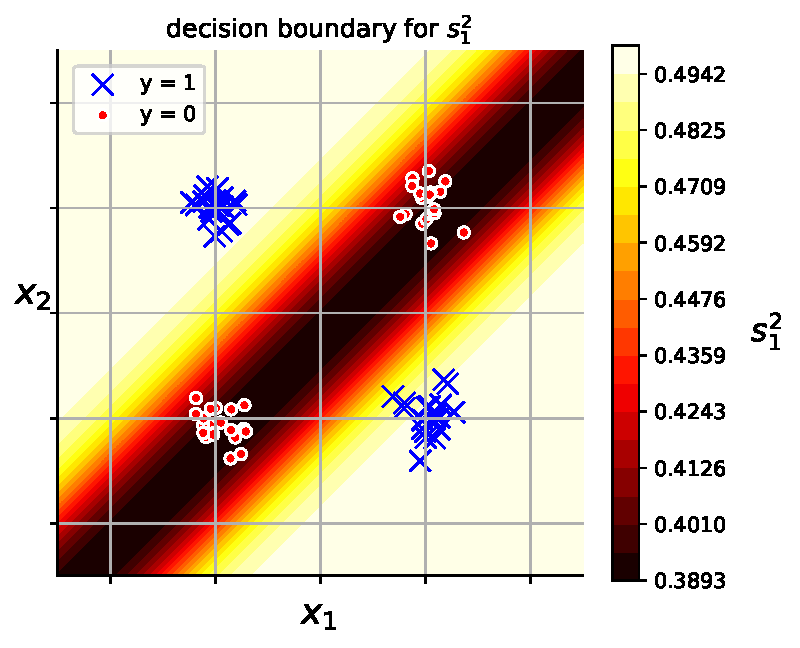
\includegraphics[width=0.4\textwidth]{img/xor_decision}
	 }
     \mode<article>{
	 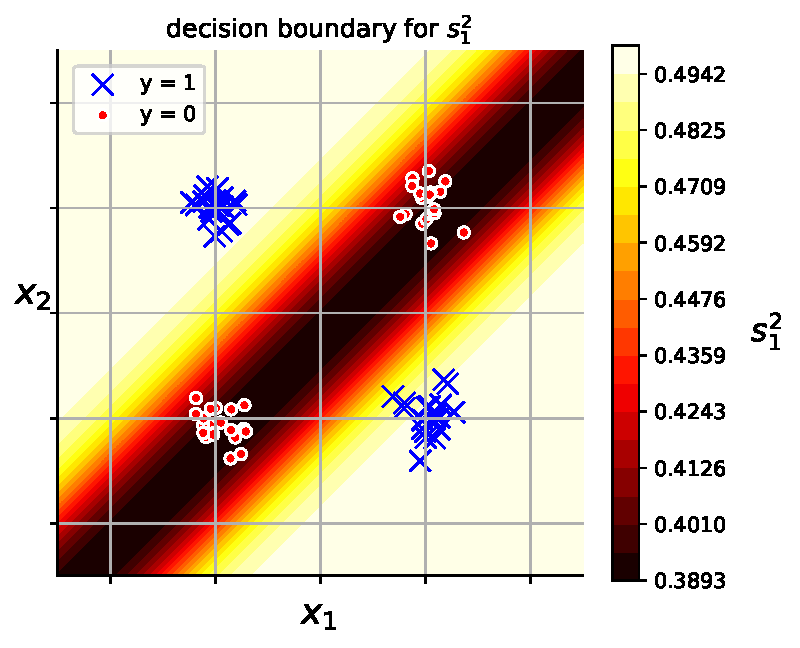
\includegraphics[width=0.35\textwidth]{img/xor_decision}
	 }
	 }%
     \begin{subfigure}[t]{0.35\textwidth}
         \centering
         \usebox{\imagebox}% Place largest image
         \caption{}
         \label{fig:xor_decisions}
     \end{subfigure}
     \slidesonly{
     \hspace{4mm}
     \begin{subfigure}[t]{0.45\textwidth}
     }
    \notesonly{
     \hspace{1mm}
     \begin{subfigure}[t]{0.38\textwidth}
     }
         \centering
         \raisebox{\dimexpr.5\ht\imagebox-.5\height}{% Raise smaller image into place
         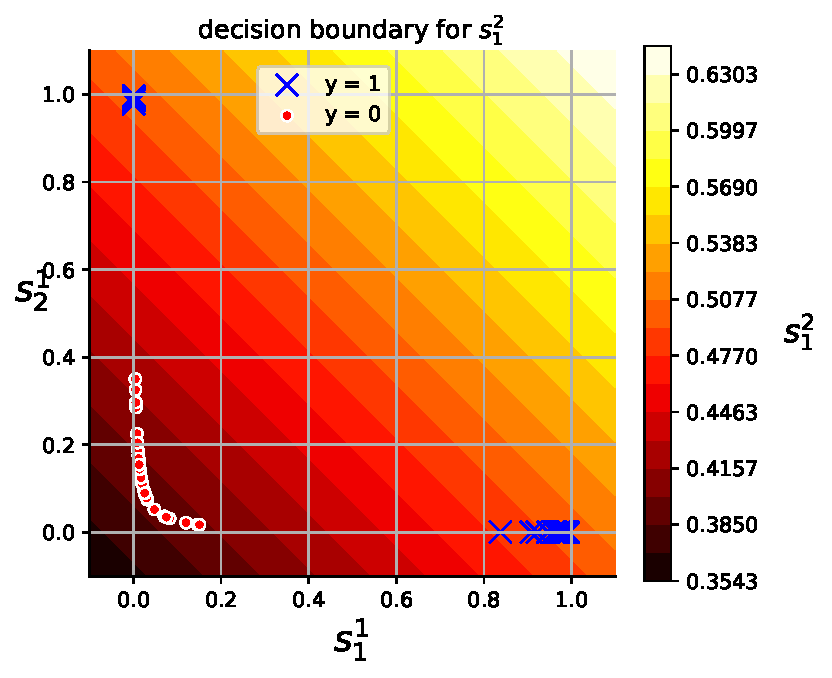
\includegraphics[width=0.9\textwidth]{img/xor_decision_s}
         }
         \caption{}
         \label{fig:xor_decisions_s}
     \end{subfigure}
	\caption{Identifying the decision boundaries.}
\end{figure}
\end{frame}

\newpage
\mode<article>{


What we are essentially describing is a Multilayered perceptron (MLP) with an architecture as illustrated in \figref{fig:xor_mlp_arch}. This MLP is made up of an output layer with a single output neuron ${\color{blue}s^2_1}$, and one hidden layer with two hidden neurons, ${\color{magenta}s^1_1}$ and ${\color{green}s^2_2}$ (the superscript denotes the layer index, the subscript denotes the neuron index within its layer). The terms ``neurons'' and ``nodes'' are treated as synonyms.
}
\begin{frame}

\begin{figure}[ht]
    \centering
	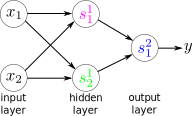
\includegraphics[width=0.4\textwidth]{img/xor_mlp_arch}
	\caption{simplified MLP architecture}
	\label{fig:xor_mlp_arch} 
\end{figure}



\end{frame}


